
\chapter{2. Linear PDEs, naively}

We start with a cliched example because it is the right place to start.

\section{A finite element method for the Poisson problem}

Let $\Omega \subset \RR^d$ be a region\marginnote{Only $d=2$ and $d=3$ are used in this book.} with boundary decomposed into well-behaved subsets $\partial_D \Omega$ and $\partial_N \Omega$ whose union is the whole boundary $\partial \Omega$.  The \emph{Poisson problem}, in strong form and including both Dirichlet and Neumann boundary conditions, is
\begin{align}
- \grad^2 u &= f \quad \text{ on } \Omega, \label{poissonstrong} \\
u &= g \quad \text{ on } \partial_D \Omega, \notag \\
\frac{\partial u}{\partial n} &= h \quad \text{ on } \partial_N \Omega \notag
\end{align}
where $\partial u/\partial n = \bn \cdot \grad u$ and $\bn$ is the outward unit normal on $\partial \Omega$.\marginnote{%
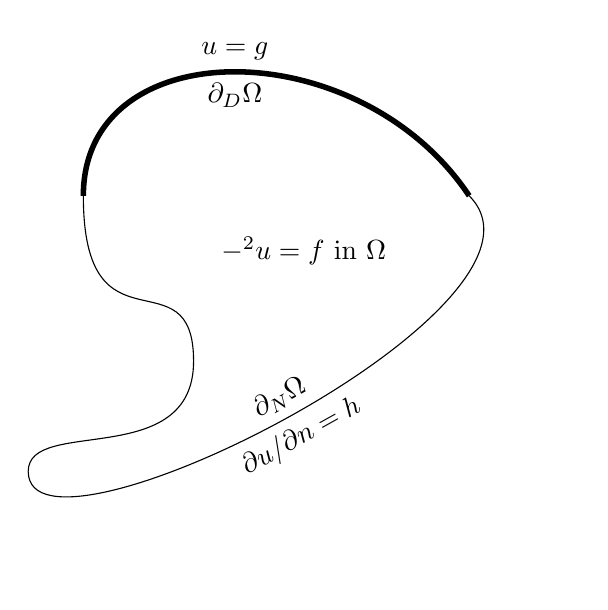
\begin{tikzpicture}[scale=0.7]
%\draw[gray,very thin] (-2,-7) grid (9,4);
\draw[line width=2pt] (0,0) .. controls (0,3) and (5,3) .. node[sloped,above] {$u=g$} node[sloped,below] {$\partial_D\Omega$} (7,0);
\draw (7,0) .. controls (9,-2) and (-1,-7) .. node[sloped,above] {$\partial_N\Omega$} node[sloped,below] {$\partial u/\partial n = h$} (-1,-5);
\draw (-1,-5) .. controls (-1,-4) and (2,-5) .. (2,-3);
\draw (2,-3) .. controls (2,-1) and (0,-3) .. (0,0);
\draw (4,-1) node {$- \grad^2 u = f$ in $\Omega$};
\end{tikzpicture}}

The data of problem \eqref{poissonstrong}, besides the region $\Omega$ and its boundary, is a \emph{source term} $f\in L^2(\Omega)$, \emph{Dirichlet data} $g\in L^2(\partial_N \Omega)$, and \emph{non-homogeneous Neumann data} $h\in L^2(\partial_N \Omega)$.  For simplicity, and so that the solution of this problem is unique if it exists \citep{Elmanetal2005}, we assume $\partial_D \Omega$ has positive measure.  All of our examples will have that property.

The Poisson problem models the distribution of temperature in a conducting object at steady state, the electrostatic potential, the equilibrium distribution from certain random walks, and many other other physical phenomena.  And it is linear, that is, if $u_1$ and $u_2$ are solutions then convex linear combinations are also solutions.  More relevantly, it is a linear problem in the sense that finite-dimensional approximations of the Poisson problem are simply matrix problems.

As \eqref{poissonstrong} is stated there may be no solution where ``$\grad^2 u$'' makes sense as a function.  In particular, there may be no $u\in C^2(\Omega)$ which is continuous up to the boundary (i.e.~$u\in C(\bar\Omega)$).  There is, however, a unique solution\sidenote{Many mathematical concepts, including a well-posedness proof that justifies this claim, are all covered by \citep{Evans}.  These are technicalities for us.  Our goal is computational performance in cases where the Poisson problem is mathematically well-behaved.} if we change to a \emph{weak formulation}.  We will state the weak formulation after defining function spaces.

Let
    $$H^1(\Omega) = \{u\in L^2(\Omega) \big| \grad u \text{ exists a.e.~and } \grad u \in L^2(\Omega)\},$$
a Sobolev space \citep{Evans}.  This space has two subsets we will use, namely functions with value $g$ and those with value $0$ on $\partial_D \Omega$, respectively, which we denote $H_g^1(\Omega)$ and $H_0^1(\Omega)$.

The weak formulation of \eqref{poissonstrong} comes from choosing any $v\in H_0^1(\Omega)$, multiplying the first equation in \eqref{poissonstrong} by $v$, and integrating by parts:
\begin{equation*}
\int_\Omega \grad u \cdot \grad v - \int_{\partial\Omega} \frac{\partial u}{\partial n} v = \int_\Omega f v.
\end{equation*}
Now,\marginnote{%
{\color{red}The main ideas} of strong and weak formulations:\begin{itemize}
\item If $u \in H_g^1(\Omega)$ solves the strong form \eqref{poissonstrong} then it solves \eqref{poissonweak} also.
\item If $u \in H_g^1(\Omega)$ solves the weak form \eqref{poissonweak} then we accept it, by definition, as a solution of the Poisson problem.\end{itemize}}
supposing we already have a classical solution $u$ of \eqref{poissonstrong}, which is in $H_g^1(\Omega)$, we use the fact that $v=0$ on $\partial_D\Omega$ and the Neumann data:
\begin{equation}
\int_\Omega \grad u \cdot \grad v = \int_\Omega f v + \int_{\partial_N\Omega} h v\quad \text{ for any } v\in H_0^1(\Omega). \label{poissonweak}
\end{equation}

Equation \eqref{poissonweak} is the weak formulation of the Poisson problem.  A key observation is that $u$ itself satisfies the Dirichlet boundary condition because it lives in $H_g^1(\Omega)$, while Neumann boundary data $h$, like the source function $f$, appears directly in \eqref{poissonweak}.

The \emph{finite element method} (FEM) comes from requiring the weak formulation for $u$ in a finite-dimensional subset of $H_g^1(\Omega)$, and for $v$ in a finite-dimensional subspace of $H_0^1(\Omega)$; more precisely, this is a \emph{Galerkin} FEM.  We will build these finite-dimensional subsets, in the current example, using a \emph{unstructured triangulation} on a region $\Omega\subset \RR^2$

To make this work, from now on we require that $\Omega$ be polygonal,\marginnote{%
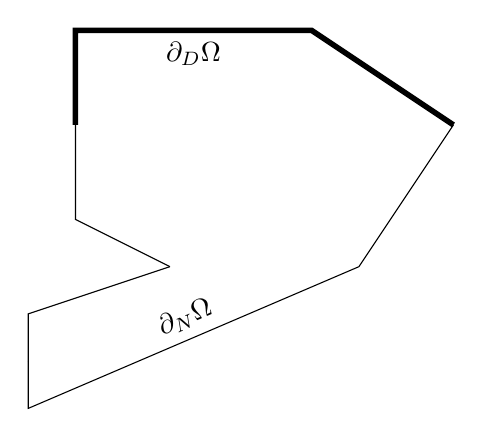
\begin{tikzpicture}[scale=0.6]
%\draw[gray,very thin] (-2,-7) grid (9,4);
\draw[line width=2pt] (0,0) -- (0,2) -- node[sloped,below] {$\partial_D\Omega$} (5,2) -- (8,0);
\draw (8,0) -- (6,-3) -- node[sloped,above] {$\partial_N\Omega$} (-1,-6) -- (-1,-5);
\draw (-1,-5) -- (-1,-4) -- (2,-3);
\draw (2,-3) -- (0,-2) -- (0,0);
\end{tikzpicture}}
 with boundary $\partial\Omega$ a closed polygon whose sides are each of positive length, and whose sides are either entirely in $\partial_D\Omega$ or in $\partial_N\Omega$.  As before, to produce a unique solution we require that $\partial_D\Omega$ contain at least one such side.

The triangulation itself is a set


\marginnote{{\color{red} Remember:} $u_h$ is the \emph{trial} function and $v_h$ are the \emph{test} functions}

%\vspace{4.0in}

\section{Getting a triangular mesh into \PETSc}

\cinputpart{c2triangle.c}{The standard preamble.}{I}{//STARTPREAMBLE}{//ENDPREAMBLE}

\cinputpart{c2triangle.c}{Determine filenames using \PETSc option processing.}{II}{//ENDPREAMBLE}{//ENDFILENAME}

\cinputpart{c2triangle.c}{Start to read ASCII files with \textsc{triangle}-generated mesh by going to rank zero processor, reading node header, and allocating accordingly.}{III}{//ENDFILENAME}{//ENDRANK0ALLOC}

\cinputpart{c2triangle.c}{On rank zero processor: Read node information.}{IV}{//ENDRANK0ALLOC}{//ENDREADNODES}

\cinputpart{c2triangle.c}{On rank zero processor: Read element information.}{V}{//ENDREADNODES}{//ENDREADELEMENTS}

\cinputpart{c2triangle.c}{On rank zero processor: Write the mesh out in \PETSc binary format.}{VI}{//ENDREADELEMENTS}{//ENDRANK0}

\cinputpart{c2triangle.c}{Re-read mesh in parallel, and write in parallel.}{VII}{//ENDRANK0}{//END}


\section{FEM method, for the Poisson equation}

\section{Preallocate a \pMat}

%\cinputfull{c2prealloc.c}{demonstrates preallocation of parallel \pMat}{}{}

\section{Assembling Poisson}

\section{Performance: convergence and scaling}

\caveat{But real-world PDEs are nonlinear.}
